\chapter{Inside the GPU: the NVIDIA A100}
\label{ch:a100}

\slides{4--11, 17--18}

This chapter follows the slides' tour of one real chip, the NVIDIA \textbf{A100} (``Ampere'' generation, 2020),
and its older relative the Kepler \textbf{K40}. Numbers for the A100 are checked against NVIDIA's
\emph{A100 Tensor Core GPU Architecture} whitepaper, the recommended reading in the course schedule. Where the slides and the
whitepaper differ, this is pointed out.

\section{The hierarchy of building blocks}

\slides{4--6}

A GPU is built like a company: many small units grouped into bigger and bigger groups. Reading from the top:

\begin{definition}{the GPU hierarchy (A100)}
\begin{itemize}
  \item The \term{GPU} contains several \term{Graphics Processing Clusters (GPCs)}.
  \item A GPC contains several \term{Texture Processing Clusters (TPCs)}.
  \item A TPC contains $2$ \term{Streaming Multiprocessors (SMs)}.
  \item An SM contains the actual execution units (FP32, INT32, FP64, Tensor Cores, \dots) together with its own registers and its own on-chip memory.
\end{itemize}
\end{definition}
The names are historical: ``texture'' comes from the graphics days. For computing, the only level
that really matters is the \textbf{SM}: it is the unit that is programmed and scheduled, and it is the unit
we will keep returning to.

% Schematic of the full GA100 chip (8 GPCs). A100 enables 7 GPCs / 108 SMs and 5 of the 6 HBM2 stacks.
\begin{figure}[ht]
\centering
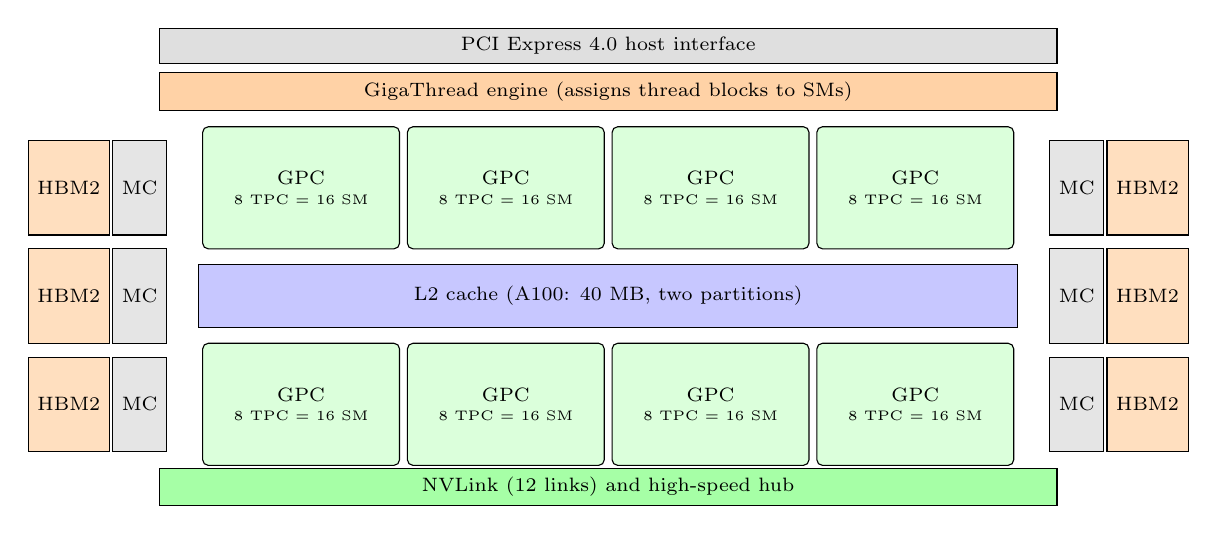
\begin{tikzpicture}[x=1cm,y=1cm,font=\scriptsize,
  gpc/.style={draw,rounded corners=2pt,fill=green!14,minimum width=2.5cm,minimum height=1.55cm,align=center},
  hbm/.style={draw,fill=orange!25,minimum width=1.0cm,minimum height=1.2cm,align=center},
  mc/.style={draw,fill=gray!20,minimum width=0.55cm,minimum height=1.2cm,align=center}]
  % top bars
  \node[draw,fill=gray!25,minimum width=11.4cm,minimum height=0.45cm] at (0,4.55) {PCI Express 4.0 host interface};
  \node[draw,fill=orange!35,minimum width=11.4cm,minimum height=0.45cm] at (0,3.97) {GigaThread engine (assigns thread blocks to SMs)};
  % GPCs top row and bottom row
  \foreach \i in {0,1,2,3}{
    \node[gpc] at (-3.9+2.6*\i,2.75) {GPC\\[-1pt]{\tiny 8 TPC $=$ 16 SM}};
    \node[gpc] at (-3.9+2.6*\i,0.0) {GPC\\[-1pt]{\tiny 8 TPC $=$ 16 SM}};
  }
  % L2
  \node[draw,fill=blue!22,minimum width=10.4cm,minimum height=0.8cm] at (0,1.375) {L2 cache (A100: 40 MB, two partitions)};
  % memory controllers and HBM left/right
  \foreach \y in {2.75,1.375,0}{
    \node[mc] at (-5.95,\y) {MC};
    \node[mc] at (5.95,\y) {MC};
    \node[hbm] at (-6.85,\y) {HBM2};
    \node[hbm] at (6.85,\y) {HBM2};
  }
  % NVLink
  \node[draw,fill=green!35,minimum width=11.4cm,minimum height=0.45cm] at (0,-1.05) {NVLink (12 links) and high-speed hub};
\end{tikzpicture}
\caption{Simplified block diagram of the full GA100 chip. The A100 product enables $7$ of the $8$ GPCs
(and not all TPCs inside them) and $5$ of the $6$ HBM2 stacks. Compare slide~5.}
\label{fig:gpu}
\end{figure}


\subsection{The numbers}

The slide says: $7$ GPCs; each GPC has $7$ or $8$ TPCs ``hence a total of $64$ TPCs''; up to $16$ SMs per GPC; ``a total of $108$ SMs''.
Table~\ref{tab:a100counts} puts the numbers together.

\begin{table}[ht]
\centering\small
\begin{tabular}{@{}lcc@{}}
\toprule
 & \textbf{Full GA100 chip} & \textbf{A100 product}\\
\midrule
GPCs & $8$ & $7$\\
TPCs per GPC & $8$ & $7$ or $8$\\
SMs per TPC & $2$ & $2$\\
SMs per GPC & $16$ & up to $16$\\
\textbf{Total SMs} & $128$ & $\mathbf{108}$\\
Total TPCs & $64$ & $54$\\
FP32 units per SM & $64$ & $64$\\
FP32 units in total & $8192$ & $6912$\\
Tensor Cores per SM & $4$ & $4$\\
Tensor Cores in total & $512$ & $432$\\
\bottomrule
\end{tabular}
\caption{The full GA100 design and the A100 product that is sold (whitepaper). Factory chips that
are ``cut down'' in this way allow dies with a few defective units to be sold.}
\label{tab:a100counts}
\end{table}

\begin{pitfall}
The slide says ``a total of $64$ TPCs'' next to ``$108$ SMs''. These two numbers do not belong
to the same chip. Since an SM pair makes a TPC, $108$ SMs means $108/2=54$ TPCs; $64$ TPCs (and $128$ SMs) is the
\emph{full} GA100 design with all $8$ GPCs. This is also why Figure~6 on slide~5 is captioned
``GA100 full GPU with $128$ SMs (A100 Tensor Core GPU has $108$ SMs)''. If a question asks for the A100, use $108$ SMs and $54$ TPCs.
\end{pitfall}

\begin{workedex}{recovering the totals}
$108$ SMs $\times$ $64$ FP32 units per SM $=6912$ FP32 units (the slide's ``$6912$ GPU cores'').
$108\times4$ Tensor Cores $=432$. The whitepaper also gives $32$ FP64 units per SM, so $108\times32=3456$ FP64 units.
Note that $7$ GPCs $\times$ $16$ SMs would give $112$; the product has only $108$ because some SMs are switched off.
\end{workedex}

\section{Inside a Streaming Multiprocessor}

\slides{7--9}

The SM is the heart of the GPU, and slide~8 is one of the most important pictures in the deck. The
slide~7 text says: each SM has $64$ FP32 cores, $4$ Tensor Cores and $192$~KB of combined shared memory and L1 data cache. Figure~\ref{fig:sm} redraws the picture.

% Schematic of one A100 SM (slides 8-9)
\begin{figure}[ht]
\centering
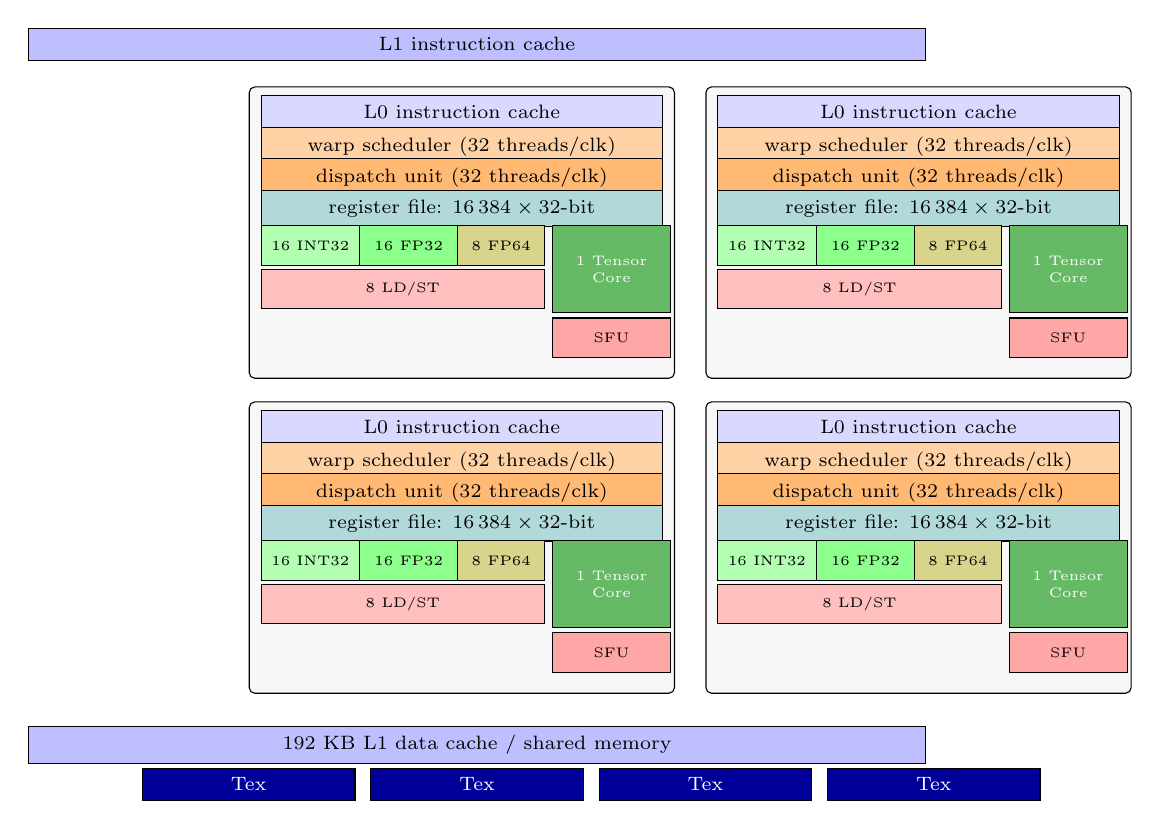
\begin{tikzpicture}[font=\scriptsize,
  part/.style={draw,rounded corners=2pt,fill=gray!6,minimum width=5.4cm,minimum height=3.7cm},
  bar/.style={draw,minimum width=5.1cm,minimum height=0.36cm,align=center},
  unit/.style={draw,minimum height=0.5cm,align=center}]
  \node[bar,fill=blue!25,minimum width=11.4cm] at (2.9,8.45) {L1 instruction cache};
  \foreach \px/\py in {0/4.2, 5.8/4.2, 0/0.2, 5.8/0.2}{
    \begin{scope}[shift={(\px,\py)}]
      \node[part,anchor=south west] at (0,0) {};
      \node[bar,fill=blue!15,anchor=north west] at (0.15,3.6) {L0 instruction cache};
      \node[bar,fill=orange!35,anchor=north west] at (0.15,3.2) {warp scheduler (32 threads/clk)};
      \node[bar,fill=orange!55,anchor=north west] at (0.15,2.8) {dispatch unit (32 threads/clk)};
      \node[bar,fill=teal!30,anchor=north west] at (0.15,2.4) {register file: $16\,384\times32$-bit};
      \node[unit,fill=green!30,minimum width=1.25cm,anchor=north west,font=\tiny] at (0.15,1.95) {16 INT32};
      \node[unit,fill=green!45,minimum width=1.25cm,anchor=north west,font=\tiny] at (1.4,1.95) {16 FP32};
      \node[unit,fill=olive!35,minimum width=1.1cm,anchor=north west,font=\tiny] at (2.65,1.95) {8 FP64};
      \node[unit,fill=green!55!black!60,minimum width=1.5cm,minimum height=1.1cm,anchor=north west,text=white,font=\tiny] at (3.85,1.95) {1 Tensor\\Core};
      \node[unit,fill=red!25,minimum width=3.6cm,anchor=north west,font=\tiny] at (0.15,1.4) {8 LD/ST};
      \node[unit,fill=red!35,minimum width=1.5cm,anchor=north west,font=\tiny] at (3.85,0.78) {SFU};
    \end{scope}
  }
  \node[bar,fill=blue!25,minimum width=11.4cm] at (2.9,-0.45) {192 KB L1 data cache / shared memory};
  \foreach \i in {0,1,2,3}{\node[bar,fill=blue!60!black,text=white,minimum width=2.7cm] at (0.0+2.9*\i-0.0,-0.95) {Tex};}
\end{tikzpicture}
\caption{One A100 SM drawn as four identical sub-partitions that share the L1/shared-memory block and the
texture units (compare slide~8). Multiplying the per-partition numbers by four gives $64$ FP32, $64$ INT32,
$32$ FP64 units, $4$ Tensor Cores and a $65\,536$-entry register file for the whole SM.}
\label{fig:sm}
\end{figure}


\subsection{Four partitions, each almost a small processor}

The SM is divided into \textbf{four identical partitions} (slide~8 shows all four; slide~9 shows two of them, enlarged). Everything with a scheduling job is replicated per partition. Each partition has:
\begin{itemize}
  \item An \textbf{L0 instruction cache} (and the SM has a shared L1 instruction cache above them), which holds the program being run.
  \item A \textbf{warp scheduler} and a \textbf{dispatch unit}, each labelled ``$32$ thread/clk'' on the slide. A \emph{warp} is a group of $32$ threads (next section); the scheduler picks a ready warp and the dispatch unit sends its next instruction to the execution units. Slide's meaning: one instruction for $32$ threads can be issued per clock per partition.
  \item A \textbf{register file} of $16\,384\times32$-bit registers ($64$~KB).
  \item The execution units: $16$ INT32 units (integer arithmetic), $16$ FP32 units (single-precision floating point), $8$ FP64 units (double precision), and $1$ Tensor Core (matrix engine, Section~\ref{sec:tensor}).
  \item $8$ load/store (LD/ST) units, which send memory requests, and a \textbf{special function unit (SFU)}, which computes things like $\sin$, $\sqrt{\ }$, $1/x$ that are too expensive for the ordinary units.
\end{itemize}
At the bottom, shared by all four partitions, sit the \textbf{$192$~KB L1 data cache / shared memory} and the \textbf{texture units} (``Tex'' on the slide, four of them).

\begin{workedex}{from one partition to the whole SM}
Per partition: $16$ FP32, $16$ INT32, $8$ FP64, $1$ Tensor Core, register file $16\,384$ entries.
Times $4$ partitions: $64$ FP32 (the slide's ``$64$ FP32 GPU cores''), $64$ INT32, $32$ FP64, $4$ Tensor Cores,
and $4\times16\,384=65\,536$ registers $=65\,536\times4$~B $=256$~KB per SM. This agrees with the whitepaper and with
the ``$64$K registers in each SMX'' on slide~14.
Over the whole chip: $108\times256$~KB $=27\,648$~KB $\approx27$~MB of registers, \emph{more than the $L2$ cache of many CPUs}.
The register file is large because each of the thousands of resident threads keeps its own variables
in it (Chapter~\ref{ch:gpumem}).
\end{workedex}

\begin{intuition}
Why does a partition with $16$ FP32 units get a scheduler that handles $32$ threads at a time? A warp has $32$ threads
but the partition has only $16$ FP32 lanes. A $32$-thread FP32 instruction therefore takes two clock cycles on that
partition's FP32 units. The scheduler is not waiting during that time, though: the A100 also has separate INT32 units, so a stream
of mixed integer and floating-point instructions from different warps can be kept running side by side.
\end{intuition}

\begin{keyidea}
An SM is \emph{not} one big core with $64$ ALUs. It is four small in-order processors, each issuing
\emph{one instruction for a whole warp} per cycle, sharing a block of fast on-chip memory.
\end{keyidea}

\section{Threads, warps and SIMT}
\label{sec:simt}

\slides{17}

Slide~17 contains the single most important phrase of the lecture: \emph{``SIMD execution (actually SIMT)''}.
The word SIMD was introduced in Chapter~\ref{ch:classify}: one instruction, many data items, executed in lock-step.
The GPU does the same but exposes it differently to the programmer.

\begin{definition}{SIMT}
\term{Single Instruction, Multiple Threads}. The programmer writes the program for \emph{one thread}, in ordinary scalar style.
The hardware runs many such threads, grouped into \term{warps} of $32$ consecutive threads. All threads of a warp are issued the same instruction in the same cycle,
each on its own data and registers, but each thread has its \emph{own} program counter state and can therefore branch independently.
\end{definition}

The hardware executes warps. The programmer thinks in threads. Compare:
\begin{center}\small
\begin{tabular}{@{}p{3.6cm}p{5.2cm}p{5.2cm}@{}}
\toprule
 & \textbf{SIMD (CPU vector unit)} & \textbf{SIMT (GPU warp)}\\
\midrule
Program written as & operations on a \emph{vector} (e.g.\ $8$ numbers per instruction) & code for a single \emph{thread}\\
Registers & one wide vector register & each thread has its own private registers\\
Branching & programmer uses masks by hand & each thread can take its own branch; hardware handles it\\
Memory access & vector load of consecutive addresses & each thread has its own address\\
\bottomrule
\end{tabular}
\end{center}

\subsection{Branch divergence}

Because the $32$ threads of a warp share one instruction stream, what happens if they disagree at an \cl{if}?
\begin{lstlisting}
if (x[i] > 0)      // some threads of the warp true, some false
    y[i] = sqrt(x[i]);
else
    y[i] = 0;
\end{lstlisting}
The hardware runs \emph{both} paths one after the other: first it executes the \cl{if} branch with the threads that said ``true'' enabled and the others switched off (masked), then the \cl{else}
branch with the opposite set enabled. Threads that are masked off simply idle.
This is \term{branch divergence}.

\begin{workedex}{cost of divergence}
Suppose the \cl{if} part takes $10$ cycles and the \cl{else} part $6$ cycles.
If all $32$ threads of the warp take the same side, the warp spends $10$ or $6$ cycles.
If the warp is split, it spends $10+6=16$ cycles, and during the first $10$ only some lanes work.
Worst case with several nested or $k$-way branches: the time is the \emph{sum} of the path times, so
utilisation can fall to $1/32$ if each of the $32$ threads takes a different path.
\end{workedex}

\begin{pitfall}
Divergence matters only \emph{within} a warp. If threads $0$--$31$ all take the \cl{if} and threads $32$--$63$ all take the \cl{else},
there is no penalty, because these are different warps and can follow different paths. So write conditions that
are constant over aligned groups of $32$ threads whenever possible, e.g.\ \cl{if (threadIdx.x / 32 == 0)} instead of \cl{if (threadIdx.x \% 2 == 0)}.
\end{pitfall}

\subsection{How the programmer's threads reach the hardware}

\slides{12}

Slide~12 (the \emph{CUDA memory spaces} picture) already shows the programmer's view that the CUDA lectures
will develop: a \term{grid} of \term{thread blocks}, each block containing threads (``Thread $(0,0)$'', ``Thread $(1,0)$'', \dots).
For the hardware you only need the following mapping:
\begin{itemize}
  \item A launch creates a grid of thread blocks. Threads of one block are always placed together on \emph{one} SM, where they can cooperate through shared memory and wait for each other at barriers.
  \item One SM may hold several blocks at once. The whitepaper lists the A100 limits: at most $1024$ threads per block, $32$ blocks, $2048$ threads (i.e.\ $64$ warps) and $255$ registers per thread on an SM.
  \item A block is cut into warps of $32$ consecutive threads: threads $0$--$31$ form warp~0, threads $32$--$63$ warp~1, etc.
  \item The chip-level scheduler (the ``GigaThread engine'' of Figure~\ref{fig:gpu}) hands blocks to SMs as they have room. Different blocks cannot be assumed to run in any particular order.
\end{itemize}

\begin{workedex}{how much work is ``in flight''?}
One SM can hold up to $2048$ threads. With $108$ SMs the A100 can have $108\times2048=221\,184$ threads resident at once,
yet it has only $6912$ FP32 units. So there are about $32$ resident threads per FP32 unit. The reason for this surplus is latency hiding (Section~\ref{sec:latency}).
\end{workedex}

\section{Tensor cores}
\label{sec:tensor}

\slides{10}

The slide gives two lines: Tensor Cores are \emph{``specialized \dots compute cores for matrix operations for AI and HPC applications''} and \emph{``perform matrix multiply and accumulate (MMA) operations''}.

\begin{definition}{matrix multiply-accumulate (MMA)}
Given small matrices $A$, $B$, $C$, the operation $D\leftarrow A\times B+C$. A Tensor Core computes a whole small block of this (for example
$16\times8$ by $8\times8$ elements) as \emph{one} hardware operation, instead of one multiply-add per instruction.
\end{definition}

Why is this useful? Matrix multiplication of two $n\times n$ matrices needs $n^{3}$ multiply-adds. Deep learning and many scientific codes are mostly matrix multiplications, so making
this one operation much faster speeds up a whole field. A Tensor Core achieves this by reading each input element once and reusing it
for many multiply-adds inside the unit, instead of fetching operands again and again for every scalar instruction (compare the reuse arguments in Chapter~\ref{ch:gpumem}).

Slide~7 states that the $4$ Tensor Cores of an SM \emph{``together deliver $1024$ FP16/FP32 operations per clock''}. This means $1024$ fused multiply-adds (FMA) per clock \emph{per SM}
(i.e.\ $256$ per Tensor Core), for the dense, non-sparse case. We can check this against the whitepaper's headline figure of $312$ TFLOPS (FP16, dense):

\begin{workedex}{checking the Tensor Core rate}
An FMA counts as $2$ floating-point operations (one multiply, one add). Boost clock: $1410$~MHz. Then
\[
 108\ \text{SMs}\times1024\ \tfrac{\text{FMA}}{\text{clk}}\times2\ \tfrac{\text{FLOP}}{\text{FMA}}\times1.41\times10^{9}\ \tfrac{\text{clk}}{\text{s}}
 \approx 3.12\times10^{14}\ \text{FLOP/s}=312\ \text{TFLOPS}.
\]
\end{workedex}

For comparison, the ordinary FP32 units:
\begin{workedex}{peak FP32 and FP64 without Tensor Cores}
FP32: $6912$ units $\times2$ FLOP (FMA) $\times1.41$~GHz $=19.5$ TFLOPS. FP64: $3456\times2\times1.41$~GHz $=9.7$ TFLOPS.
These match the whitepaper's table. So for FP16 matrix work the Tensor Cores are about $312/19.5=16$ times faster than the ordinary FP32 pipeline.
\end{workedex}

The whitepaper lists the Tensor Core peak rates for several number formats; the lower the precision, the higher the rate.
\begin{center}\small
\begin{tabular}{@{}lrr@{}}
\toprule
\textbf{Format on the Tensor Core} & \textbf{Dense peak} & \textbf{With structured sparsity}\\
\midrule
FP64 & $19.5$ TFLOPS & ---\\
TF32 & $156$ TFLOPS & $312$ TFLOPS\\
FP16 / BF16 & $312$ TFLOPS & $624$ TFLOPS\\
INT8 & $624$ TOPS & $1248$ TOPS\\
INT4 & $1248$ TOPS & $2496$ TOPS\\
\bottomrule
\end{tabular}
\end{center}
\emph{Structured sparsity} is an Ampere feature: if the weights of a neural network are pruned in a fixed pattern (two of every four values are zero), the hardware skips the zeros and doubles the rate.

\begin{pitfall}
The whitepaper's comparison table prints ``$42$'' Tensor Cores per SM for the A100. This is a typographical slip in the document: the text says four per SM, and $432$ total $/\,108$ SMs $=4$.
\end{pitfall}

\section{The older generation: Kepler K40 (SMX)}

\slides{11, 17--18}

The slides also use the \textbf{Kepler K40} (2013) as a second example. Kepler calls its multiprocessor an \textbf{SMX} (``extreme'' SM); the slides use SMX and SM
interchangeably when discussing memory, but note the hardware difference. On the slides:
\begin{itemize}
  \item GPU cores are called \textbf{streaming processors (SPs)}; they are grouped into SMXs. This grouping ``promotes coarse and fine-level parallelism'': coarse across SMXs (different blocks), fine within an SMX (threads of a block).
  \item The K40 has $15$ SMXs of $192$ SP cores each, a total of $15\times192=2880$ SP cores.
  \item Each SMX has $65\,536$ registers, $192$ SP cores, $64$ DP (double-precision) cores, $32$ special function units, $32$ load/store units and $16$ texture filtering units.
  \item The clock is $1.065$~GHz, ``light-weight'' compared with a CPU; this is typical for GPUs (the A100 boosts to $1.41$~GHz).
\end{itemize}

\begin{center}\small
\begin{tabular}{@{}lcc@{}}
\toprule
 & \textbf{Kepler K40 (slides)} & \textbf{A100 (slides + whitepaper)}\\
\midrule
Multiprocessors & $15$ SMX & $108$ SM\\
FP32 cores per multiprocessor & $192$ & $64$\\
FP32 cores in total & $2880$ & $6912$\\
Registers per multiprocessor & $64$K & $64$K\\
Double-precision units per multiprocessor & $64$ & $32$\\
Shared memory + L1 per multiprocessor & $64$~KB & $192$~KB\\
Tensor Cores & none & $4$ per SM\\
Device memory & $12$~GB & $40$~GB (slides: $80$~GB model)\\
\bottomrule
\end{tabular}
\end{center}
Observe the trend: each generation puts \emph{more, smaller} multiprocessors on the chip and more on-chip memory per multiprocessor,
while the number of registers per multiprocessor stayed the same.

\begin{intuition}
Compare Figure~\ref{fig:sm} with slide~11. The K40 SMX is one big sea of $192$ cores with four schedulers in front of them.
The A100 SM is four self-contained quarters. Splitting the unit into partitions keeps the wiring between a scheduler and its execution units short
and simple, and makes it cheaper to add features such as a Tensor Core to each quarter.
\end{intuition}

\section*{Exercises}
\begin{enumerate}[label=\textbf{\thechapter.\arabic*},leftmargin=*]
  \item List the levels of the A100 hierarchy from the GPU down to an FP32 unit, and give how many of each lower-level component sit in one higher-level component.
  \item The slide says ``a total of $64$ TPCs'' and ``a total of $108$ SMs''. Explain why both cannot be true for the A100, and give the correct number of TPCs.
  \item Starting from one SM partition ($16$ FP32, $8$ FP64, $1$ Tensor Core, $16\,384$ registers), derive the per-SM and per-chip numbers of FP32 units, FP64 units, Tensor Cores and register-file size ($108$ SMs).
  \item Compute the peak FP32 rate of the A100 in TFLOPS at $1.41$~GHz. Why do we multiply by $2$?
  \item A warp executes \cl{if (tid \% 4 == 0) A(); else B();}, where \cl{A} takes $20$ cycles and \cl{B} takes $30$. How many cycles does the warp take? What fraction of the thread-slots do useful work while \cl{A} runs? Rewrite the condition so that there is no divergence for a block of $128$ threads (keeping the same amount of work for each path).
  \item Explain SIMT and say how it differs from the SIMD vector unit of a CPU. Why is it still ``lock-step'' execution?
  \item Starting from the claim of $1024$ FMA per clock per SM, reproduce the $312$ TFLOPS figure, and then compute how many times faster the FP16 Tensor Core rate is than the FP32 CUDA-core rate.
  \item How many warps can be resident on one SM, given the limit of $2048$ threads? How many per partition if they are spread evenly?
\end{enumerate}
